% Solar Filament Segmentation Challenge 2026: technical report.
% Body is template-agnostic: paste sections into the organizers' Overleaf template if required.
\documentclass[10pt,twocolumn]{article}
\usepackage[margin=0.7in]{geometry}
\usepackage{graphicx,booktabs,amsmath,xcolor,tikz,caption}
\usepackage[hidelinks]{hyperref}
\usetikzlibrary{positioning,arrows.meta,fit}
\captionsetup{font=small,skip=3pt}
\setlength{\textfloatsep}{8pt}
\setlength{\floatsep}{6pt}

\title{A Proposal, Refine and Merge Cascade for Solar Filament Instance Segmentation}
\author{Team TODO: Richmond Azumah, Charan TODO, Hassan TODO, Sheikh TODO, Varshi TODO\\
\small Advanced Machine Learning, Solar Filament Segmentation Challenge 2026}
\date{}

\begin{document}
\maketitle

\begin{abstract}
We segment individual solar filaments in 2048$\times$2048 GONG H$\alpha$ full-disk images and score them
with Panoptic Quality (PQ). Our pipeline has three learned stages: a YOLO11l-seg instance proposer, a
dense ConvNeXt U-Net whose filament and centerline probabilities guide a second stage, and an
instance-conditioned ResNet-34 refiner that redraws each proposal's mask and predicts its own IoU. A
second, independent U-Net trained at native resolution supplies extra proposals that are refined the
same way and merged by score-ranked overlap resolution. On a leak-free 5-fold out-of-fold evaluation
over all 707 training images the final system reaches PQ 0.460 (YOLO alone 0.421; two human
annotators agree at 0.344), and it scores 0.40 on the public leaderboard.
\end{abstract}

\section{Task, data and evaluation}
The training set has 707 full-disk images with 1 to 3 independent annotation sets each (1,154 sets,
8,199 filament polygons); the test set has 180 images. A prediction matches a ground-truth filament when
their IoU exceeds 0.5, and
$\mathrm{PQ}=\sum_{\mathrm{TP}}\mathrm{IoU}/(|\mathrm{TP}|+\tfrac12|\mathrm{FP}|+\tfrac12|\mathrm{FN}|)
=\mathrm{SQ}\times\mathrm{RQ}$.
Because a hidden test label is one annotator's set, we score every image against each of its annotation
sets and average, which estimates the expected leaderboard PQ. We also report the share of ground-truth
filaments split across two or more predictions (one-to-many, fragmentation) and the share of
predictions that swallow two or more filaments (many-to-one, over-merging). Annotators disagree
strongly: one annotator scored against the others reaches only PQ 0.344.

\paragraph{Validation.} All annotation sets of a physical image stay in one fold. We use 5 folds
stratified by observing site and filament-count quartile, and every number below is out-of-fold (OOF):
each image is predicted by models that never saw it, and thresholds are tuned once on the pooled 707
images. Tuning on a single 142-image fold was 0.004 optimistic, and the public leaderboard (two decimals,
about 90 images) cannot separate variants within 0.01, so pooled OOF PQ drives every decision.

\paragraph{Rules.} Only the provided test images are used at inference. The JSON spine and chirality
fields are never used; centerlines are derived by skeletonizing masks.

\section{Method}
\begin{figure*}[t]
\centering
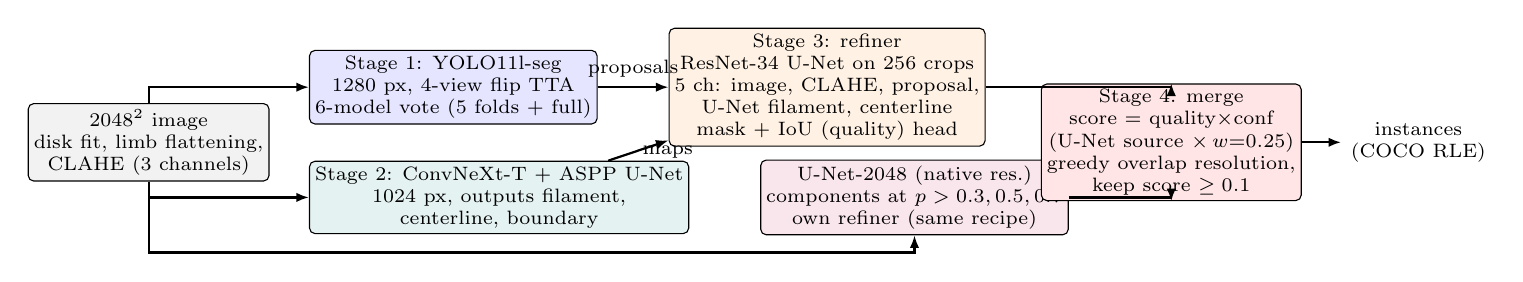
\begin{tikzpicture}[node distance=4mm and 5mm, every node/.style={font=\scriptsize, align=center},
  box/.style={draw, rounded corners=2pt, minimum height=8mm, inner sep=2pt, fill=#1!10}, box/.default=gray,
  ar/.style={-{Latex[length=1.6mm]}, thick}]
\node[box] (img) {2048$^2$ image\\disk fit, limb flattening,\\CLAHE (3 channels)};
\node[box=blue, right=of img, yshift=7mm] (yolo) {Stage 1: YOLO11l-seg\\1280 px, 4-view flip TTA\\6-model vote (5 folds + full)};
\node[box=teal, right=of img, yshift=-7mm] (unet) {Stage 2: ConvNeXt-T + ASPP U-Net\\1024 px, outputs filament,\\centerline, boundary};
\node[box=orange, right=of yolo, xshift=4mm] (ref) {Stage 3: refiner\\ResNet-34 U-Net on 256 crops\\5 ch: image, CLAHE, proposal,\\U-Net filament, centerline\\mask + IoU (quality) head};
\node[box=purple, right=of unet, xshift=4mm] (u2) {U-Net-2048 (native res.)\\components at $p>0.3,0.5,0.7$\\own refiner (same recipe)};
\node[box=red, right=of ref, xshift=2mm, yshift=-7mm] (merge) {Stage 4: merge\\score $=$ quality$\times$conf\\(U-Net source $\times\,w{=}0.25$)\\greedy overlap resolution,\\keep score $\ge 0.1$};
\node[right=of merge] (out) {instances\\(COCO RLE)};
\draw[ar] (img) |- (yolo); \draw[ar] (img) |- (unet);
\draw[ar] (yolo) -- node[above]{proposals} (ref);
\draw[ar] (unet) -- node[right, pos=0.4]{maps} (ref);
\draw[ar] (img.south) |- ++(0,-9mm) -| (u2.south);
\draw[ar] (ref) -| (merge); \draw[ar] (u2) -| (merge); \draw[ar] (merge) -- (out);
\end{tikzpicture}
\caption{Pipeline. Every learned stage is trained 5 times (one per held-out fold) plus once on all data;
the test set uses the fold models and the full model together.}
\label{fig:pipe}
\end{figure*}

\paragraph{Preprocessing and targets.} We fit the solar disk, divide out radial limb darkening and stack
the raw, limb-flattened and CLAHE images as three channels, with the sky set to zero. Instances from
different annotation sets are clustered (IoU $>0.2$ or $>50\%$ cover); a consensus target keeps a filament
drawn by at least half of the image's annotators.

\paragraph{Stage 1: proposals.} YOLO11l-seg (27.6M parameters, COCO-pretrained, one class) is trained on
the consensus targets at 1280 px (median filament width is about 11 px at 2048) for 60 epochs (AdamW,
cosine, 180$^\circ$ rotations, flips, mosaic 0.5). Inference uses 4 flip views merged by mask voting; for
the test set the 5 fold models and the full model vote. Every instance with confidence $\ge 0.05$ is
kept as a proposal, so the later stages decide what survives.

\paragraph{Stage 2: dense maps.} A U-Net with a ConvNeXt-tiny encoder and a residual ASPP block sees the
whole disk at 1024 px and predicts three maps: filament (soft target equal to the fraction of annotators
marking the pixel), centerline (dilated skeletons) and boundary. The loss combines weighted BCE, batch
soft Dice and clDice on the filament map, plus BCE on centerline and boundary. Its OOF maps feed the
refiner.

\paragraph{Stage 3: instance-conditioned refiner.} For each proposal we crop a square around its box with
1.5$\times$ context, resize it to 256 px and stack five channels: two image channels, the proposal mask,
and the U-Net filament and centerline probabilities. A ResNet-34 U-Net redraws the mask and a scalar head
predicts the IoU of that mask with the matched filament (0 for false positives). Training mixes
corrupted ground-truth masks (down-up sampling, erosion, dilation, shifts, dropped segments, bleeding into
neighbours), real OOF YOLO proposals matched at IoU $>0.2$, and unmatched proposals as negatives with an
empty target. Loss: BCE + Dice on the mask, smooth L1 on quality; 60 epochs; D4 test-time augmentation.
The fold refiners and the full refiner average their outputs on the test set.

\paragraph{Stage 4: second source and merge.} YOLO misses about a third of the filaments. A second U-Net
with the same architecture, trained at native 2048 px on 1024 px crops, is cut into connected components
at three thresholds; each component is refined by its own refiner trained with the same recipe on these
maps. Both refined sets are ranked by quality $\times$ confidence, with the second source down-weighted by
$w$, and resolved greedily: a lower-ranked instance is dropped when less than half of it remains uncovered.
We keep instances with score $\ge 0.1$ and area $\ge 150$ px.

\section{Results}
\begin{table}[t]
\centering\small\setlength{\tabcolsep}{3pt}
\caption{Pooled 5-fold OOF results on all 707 training images (1:m one-to-many, m:1 many-to-one).}
\label{tab:main}
\begin{tabular}{lccccccc}
\toprule
Stage & PQ & SQ & RQ & Prec. & Rec. & 1:m & m:1 \\
\midrule
Human agreement & 0.344 & 0.635 & 0.542 & 0.542 & 0.542 & 2.9\% & 2.9\% \\
YOLO11l-seg & 0.421 & 0.662 & 0.635 & 0.669 & 0.605 & 1.5\% & 3.9\% \\
YOLO + refiner & 0.458 & \textbf{0.684} & 0.670 & \textbf{0.726} & 0.622 & \textbf{1.2\%} & 3.6\% \\
U-Net-2048 + refiner & 0.452 & 0.682 & 0.663 & 0.686 & 0.641 & 3.3\% & \textbf{2.4\%} \\
Union (final) & \textbf{0.460} & 0.682 & \textbf{0.674} & 0.698 & \textbf{0.653} & 2.4\% & 3.2\% \\
\bottomrule
\end{tabular}
\end{table}

Table~\ref{tab:main} shows the stages. The refiner is the largest single gain (+0.037 PQ), mostly from
recognition: its quality head discards false positives that YOLO's confidence cannot separate, so
precision rises from 0.669 to 0.726 and recall still gains (0.605 to 0.622). The merge then adds recall
(0.622 to 0.653) at a small cost in precision. Fragmentation and over-merging stay below 4\% at
every stage; the merge raises fragmentation slightly (1.2\% to 2.4\%) because a U-Net component can cover
part of a filament that a YOLO instance also covers. Every system exceeds the human agreement level, because it is scored against all annotators
and predicts the filaments most of them draw. Table~\ref{tab:fold}: the refiner gain holds on every fold and the merge helps on 4 of 5.

\begin{table}[t]
\centering\small\setlength{\tabcolsep}{4pt}
\caption{OOF PQ per fold.}
\label{tab:fold}
\begin{tabular}{lcccc}
\toprule
Fold ($n$) & YOLO & +refiner & U-Net-2048 & Union \\
\midrule
0 (142) & 0.417 & 0.452 & 0.435 & \textbf{0.456} \\
1 (142) & 0.420 & \textbf{0.458} & 0.449 & 0.453 \\
2 (141) & 0.405 & 0.444 & 0.448 & \textbf{0.450} \\
3 (141) & 0.427 & 0.474 & 0.470 & \textbf{0.477} \\
4 (141) & 0.434 & 0.462 & 0.455 & \textbf{0.463} \\
\midrule
Pooled (707) & 0.421 & 0.458 & 0.452 & \textbf{0.460} \\
\bottomrule
\end{tabular}
\end{table}

\begin{table}[t]
\centering\small\setlength{\tabcolsep}{3pt}
\caption{Ablations. Top: fold 0 (142 images, settings tuned on fold 0). Bottom: pooled 707-image OOF.}
\label{tab:abl}
\begin{tabular}{lcc}
\toprule
Variant & OOF PQ & Public \\
\midrule
U-Net alone (stage 2) & 0.406 & \\
YOLO11l-seg alone & 0.417 & 0.35 \\
\quad + refiner, 30 epochs, hflip TTA & 0.446 & \\
\quad + endpoint-bridging fusion & 0.447 & 0.40 \\
MeshNet refiner (7.5k params) & 0.448 & \\
ResNet-34 refiner, 60 epochs, D4 & 0.456 & \\
\quad + MeshNet ensemble, 6-model proposals & 0.457 & 0.39 \\
\midrule
YOLO + refiner (6-refiner vote) & 0.458 & 0.39 \\
\quad U-Net maps trained 50 instead of 30 epochs & 0.458 & \\
\quad + own U-Net proposals ($w=0.25$) & 0.442 & \\
U-Net-2048 + refiner alone & 0.452 & 0.39 \\
YOLO + refiner + U-Net-2048, $w=1.0$ & 0.451 & \\
YOLO + refiner + U-Net-2048, $w=0.25$ (final) & \textbf{0.460} & \textbf{0.40} \\
\bottomrule
\end{tabular}
\end{table}

\paragraph{Ablations (Table~\ref{tab:abl}).} Endpoint-bridging fusion of broken filaments adds only 0.001
once the refiner is in, because splitting is already rare. Training the U-Net longer improved its own PQ on
every fold but did not move the final PQ: the refiner, not its guidance maps, is the bottleneck. Proposals
cut from our own U-Net hurt (0.442): they overlap the YOLO proposals the refiner already sees and mostly add
false positives. The native-resolution U-Net errs differently, and at a quarter of the YOLO weight its
refined instances fill gaps without displacing better masks; at equal weight they do (0.451).
Figure~\ref{fig:thr}: a low weight needs a low score threshold, and a high weight cannot recover the loss
at any threshold.

\begin{figure}[t]
\centering
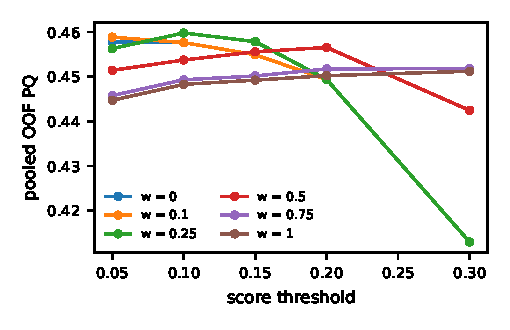
\includegraphics[width=\linewidth]{fig_threshold.pdf}
\caption{Pooled OOF PQ against the score threshold, for each weight $w$ of the U-Net-2048 source
(best min area per point).}
\label{fig:thr}
\end{figure}

\begin{figure*}[t]
\centering
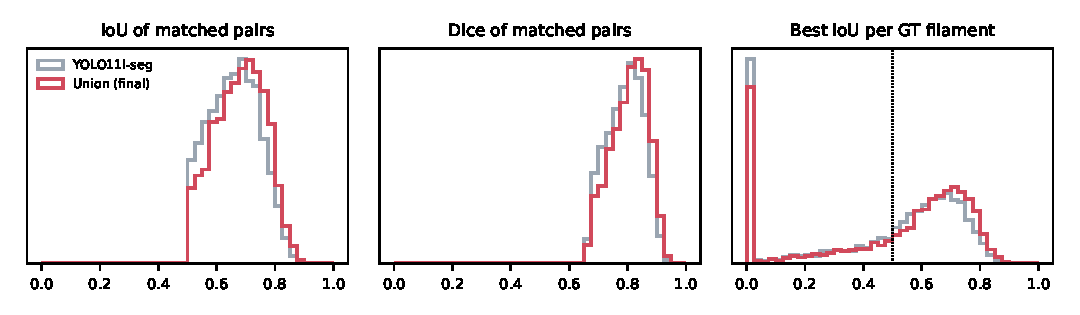
\includegraphics[width=0.92\textwidth]{fig_distributions.pdf}
\caption{Distributions over all 707 OOF images and all annotation sets. Left, middle: IoU and Dice of
matched pairs. Right: best IoU of each ground-truth filament with any prediction (left of the dotted
line: missed).}
\label{fig:dist}
\end{figure*}

\paragraph{Mask quality (Figure~\ref{fig:dist}).} The refiner shifts the whole distribution of matched IoU upward: the median rises from 0.662 to 0.685 (Dice 0.796 to 0.813) and the lower quartile from 0.594 to 0.614. The merge mainly adds matches: 5,024 matched pairs for YOLO against 5,435 for the final system, and the share of ground-truth filaments that no prediction covers at IoU $>0.5$ falls from 38.7\% to 33.7\%. Most of the remaining misses have no overlapping prediction at all (the spike at 0), so they are detection failures rather than boundary errors.

\begin{figure*}[t]
\centering
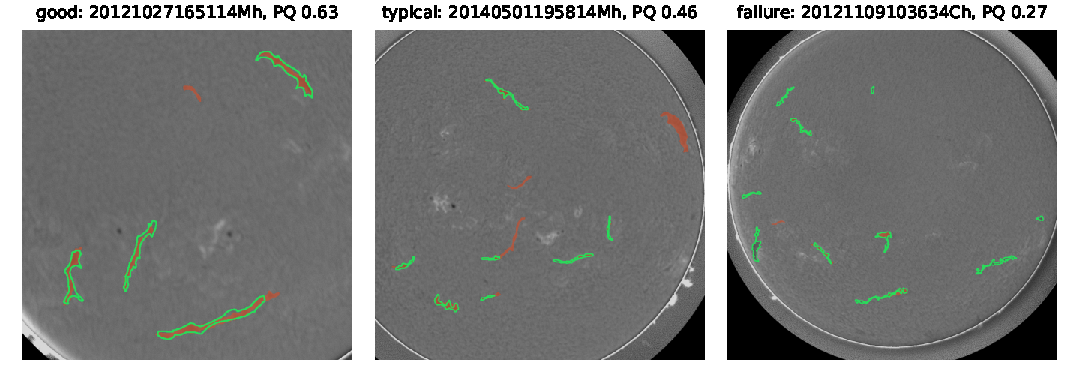
\includegraphics[width=0.92\textwidth]{fig_qualitative.pdf}
\caption{Final model on OOF images at the 95th, 50th and 5th percentile of per-image PQ (among images with
at least 4 filaments). Red: predictions; green outline: first annotation set (PQ averages over all sets).}
\label{fig:qual}
\end{figure*}

\paragraph{Qualitative (Figure~\ref{fig:qual}).} Long, high-contrast filaments are segmented with close
boundaries. Typical errors are faint or fragmented filaments near the limb that only some annotators draw,
and clusters of short dark features that annotators group differently, which also limits human agreement.

\section{Efficiency}
On Kaggle (2$\times$ T4), one YOLO fold model trains in 1.5 h (60 epochs at 1280 px), one U-Net fold in
about 1 h (30 epochs, 2 min each) and one refiner in 72 min (60 epochs, crops cached in memory). At test
time the refiner stage dominates: six refiners with D4 augmentation take 10 min for the 180 test images
(3.4 s per image); the merge runs on CPU.

\section{Discussion and limitations}
OOF PQ exceeds public PQ by about 0.06 for every model we submitted, so it is not caused by threshold selection
on OOF. Part of it is distribution shift: test images come slightly more often from 2019--2022 (12\% against
9\%), years on which our OOF PQ is lowest (0.36), but this explains only about 0.005. Public notebooks
report the same gap, which is consistent with sparser single-annotator test labels.
The public board ranked our final variants as 0.39 to 0.40, within its resolution. Recall remains the weak
side (about 0.65): faint filaments that only some annotators mark are the main loss. Code, pinned
requirements, weights and an end-to-end notebook: \url{https://github.com/hsfcoulibaly/aml_project}
(\texttt{Azumah/}).

\end{document}
